\documentclass[a4paper]{Template/LaTeX_Templates/waica}

\usepackage[T1]{fontenc}
\usepackage{graphicx}
\usepackage{booktabs}
\usepackage{multirow}
\usepackage{amsmath}
\usepackage{url}
\setlength{\emergencystretch}{1em}
\raggedbottom

\begin{document}

\title{Agentic-VLA: Inference-Time Process Control for Long-Horizon Vision-Language-Action Policies}
\author{}
\institute{}

% Double-blind version for review.

\maketitle

\begin{abstract}
Vision-language-action (VLA) models have substantially advanced robot manipulation, yet even strong fine-tuned policies remain brittle on long-horizon tasks. In many such failures, the missing capability is no longer atomic control but \emph{execution process control}: the policy can execute local skills, yet it struggles to bridge subtask transitions, maintain progress through off-nominal states, and recover after local derailments. We present \textbf{Agentic-VLA}, an inference-time augmentation framework that equips a frozen fine-tuned VLA policy with three external modules: a \textit{Transition Agent}, a lightweight \textit{scene-prior and memory module}, and a \textit{Critic/Retry module}. Rather than retraining the backbone, Agentic-VLA wraps the original policy server with a modular, auditable execution loop. We study the framework through rollouts in the official LIBERO simulator, focusing on the completed head-to-head comparison on \texttt{libero\_10}. Against a strong verified \texttt{pi05\_libero} baseline at 90.0\% success (180/200), the completed refined Full Agentic-VLA run reaches 92.5\% (185/200), with the dominant weak task improving from 55.0\% to 75.0\%. The resulting picture is encouraging but uneven: transition handling is the most stable gain source, scene priors and memory provide task-dependent benefit, and the current critic remains under-activated. We therefore interpret Agentic-VLA conservatively as a practical process-control layer for strong frozen VLAs rather than a complete solution to long-horizon robustness.
\end{abstract}

\section{Introduction}

Vision-language-action (VLA) models have emerged as a central paradigm for embodied manipulation by coupling perception, language grounding, and low-level control within a single policy. From early large-scale systems such as RT-1 and RT-2 to open and generalist stacks including Open X-Embodiment, RoboFlamingo, Octo, OpenVLA, $\pi_0$, and $\pi_{0.5}$, recent progress has made it increasingly practical to deploy strong instruction-following policies across diverse robotic settings \cite{rt1,rt2,openx,roboflamingo,octo,openvla,pi0,pi05,fast,greenvla,everydayvla}. Modern VLAs can therefore be highly competent on short-horizon manipulation once the backbone and data pipeline are strong enough.

The next barrier, however, is not simple reactive competence. In long-horizon manipulation, many rollouts still fail even when the policy already possesses the required atomic skills. Benchmarks such as CALVIN and LIBERO make this gap explicit by requiring skill chaining, temporal coherence, and recovery from off-nominal states \cite{calvin,libero}. A broad range of reasoning-oriented and hierarchical systems, including SayCan, PaLM-E, Code as Policies, VoxPoser, COME-robot, Hi Robot, OneTwoVLA, Long-VLA, and RoboCerebra, points to the same conclusion: long-horizon success depends not only on a strong action model, but also on process control, planning, and feedback handling \cite{saycan,palme,codeaspolicies,voxposer,come,hirobot,onetwovla,longvla,robocerebra}. For strong fine-tuned VLAs that are already near saturation on simpler tasks, the more practical question is therefore narrower: can a \emph{lightweight, auditable, deployment-compatible} process-control layer still produce measurable gains on difficult long-horizon rollouts?

This motivates the central question of the paper: once a strong \emph{fine-tuned} VLA policy already performs well on in-domain short-horizon tasks, what is the most effective way to repair its remaining long-horizon weaknesses? One option is to continue scaling the backbone, collecting more robot data, or redesigning the training objective. Another is to attach external process-control mechanisms at inference time. The latter is appealing because it preserves the underlying policy while providing a modular route to targeted improvement.

Recent work suggests that agentic or reasoning-based interventions can help. ECoT and Fast ECoT introduce explicit embodied reasoning before action generation \cite{ecot,fastecot}; MemoryVLA studies perceptual-cognitive memory in VLA execution \cite{memoryvla}; VLA$^2$ and ManiAgent integrate external agentic modules for unseen concepts or broader manipulation \cite{vla2,maniagent}; Sci-VLA targets state gaps in long-horizon scientific workflows \cite{scivla}; and FailSafe and Guardian emphasize failure detection and recovery through visual reasoning \cite{failsafe,guardian}. Yet many of these systems either retrain the policy, rely on custom task sets, emphasize open-world reasoning, or do not cleanly separate overall gains from the specific process-control mechanism that produces them. This leaves a practical systems question unresolved: can a strong frozen policy be improved by a modular inference-time wrapper whose behavior remains inspectable at the level of individual rollouts?

In this paper, we study a narrower but practically important setting: \emph{can a strong frozen fine-tuned VLA policy on LIBERO be improved through modular inference-time process control?} We instantiate this idea as \textbf{Agentic-VLA}, an augmentation framework that wraps a baseline \texttt{pi05\_libero} policy with three complementary mechanisms. A \textit{Transition Agent} detects stalled progress and inserts short reconnection motions to bridge subtask discontinuities. A lightweight \textit{scene-prior and memory module} injects structured hints such as approach geometry, force bias, and task-specific priors. A \textit{Critic/Retry module} periodically evaluates progress, attributes likely failure modes, and triggers recovery or retry prompts when the rollout appears to have derailed. As summarized in Figure~\ref{fig:method_overview}, these modules operate entirely at inference time around the original policy server. The resulting system is neither a new backbone nor a hidden retraining recipe; it is an external process-control layer for stabilizing long-horizon execution while preserving auditability.

We evaluate Agentic-VLA through rollouts in the official LIBERO simulator. We focus on the completed \texttt{libero\_10} comparison between the strong baseline and the refined Full Agentic-VLA system because this is the only setting in our study for which the main comparison is both complete and directly aligned with the paper's central question. \texttt{libero\_10} is also the most revealing case for our hypothesis: the \texttt{pi05\_libero} baseline already performs strongly, yet it still exhibits non-trivial weaknesses on long-horizon composite tasks. It therefore provides an appropriate setting for testing whether execution-time process control can improve an already strong policy.

Our contributions are three-fold:
\begin{enumerate}
\item We propose Agentic-VLA, an inference-time agentic augmentation framework that enhances a frozen fine-tuned VLA policy with explicit process-control mechanisms for long-horizon manipulation.
\item We instantiate three complementary modules---Transition, scene priors and memory, and Critic/Retry---within a unified execution loop around a strong frozen \texttt{pi05\_libero} policy, using conservative implementation choices that prioritize auditability over architectural novelty.
\item We build a real-rollout evaluation protocol in the official LIBERO simulator, centered on \texttt{libero\_10}, and organize the evidence hierarchy into a completed main comparison, targeted weak-task diagnosis, and explicitly out-of-scope ongoing system extensions.
\end{enumerate}

\begin{figure}[t]
\centering
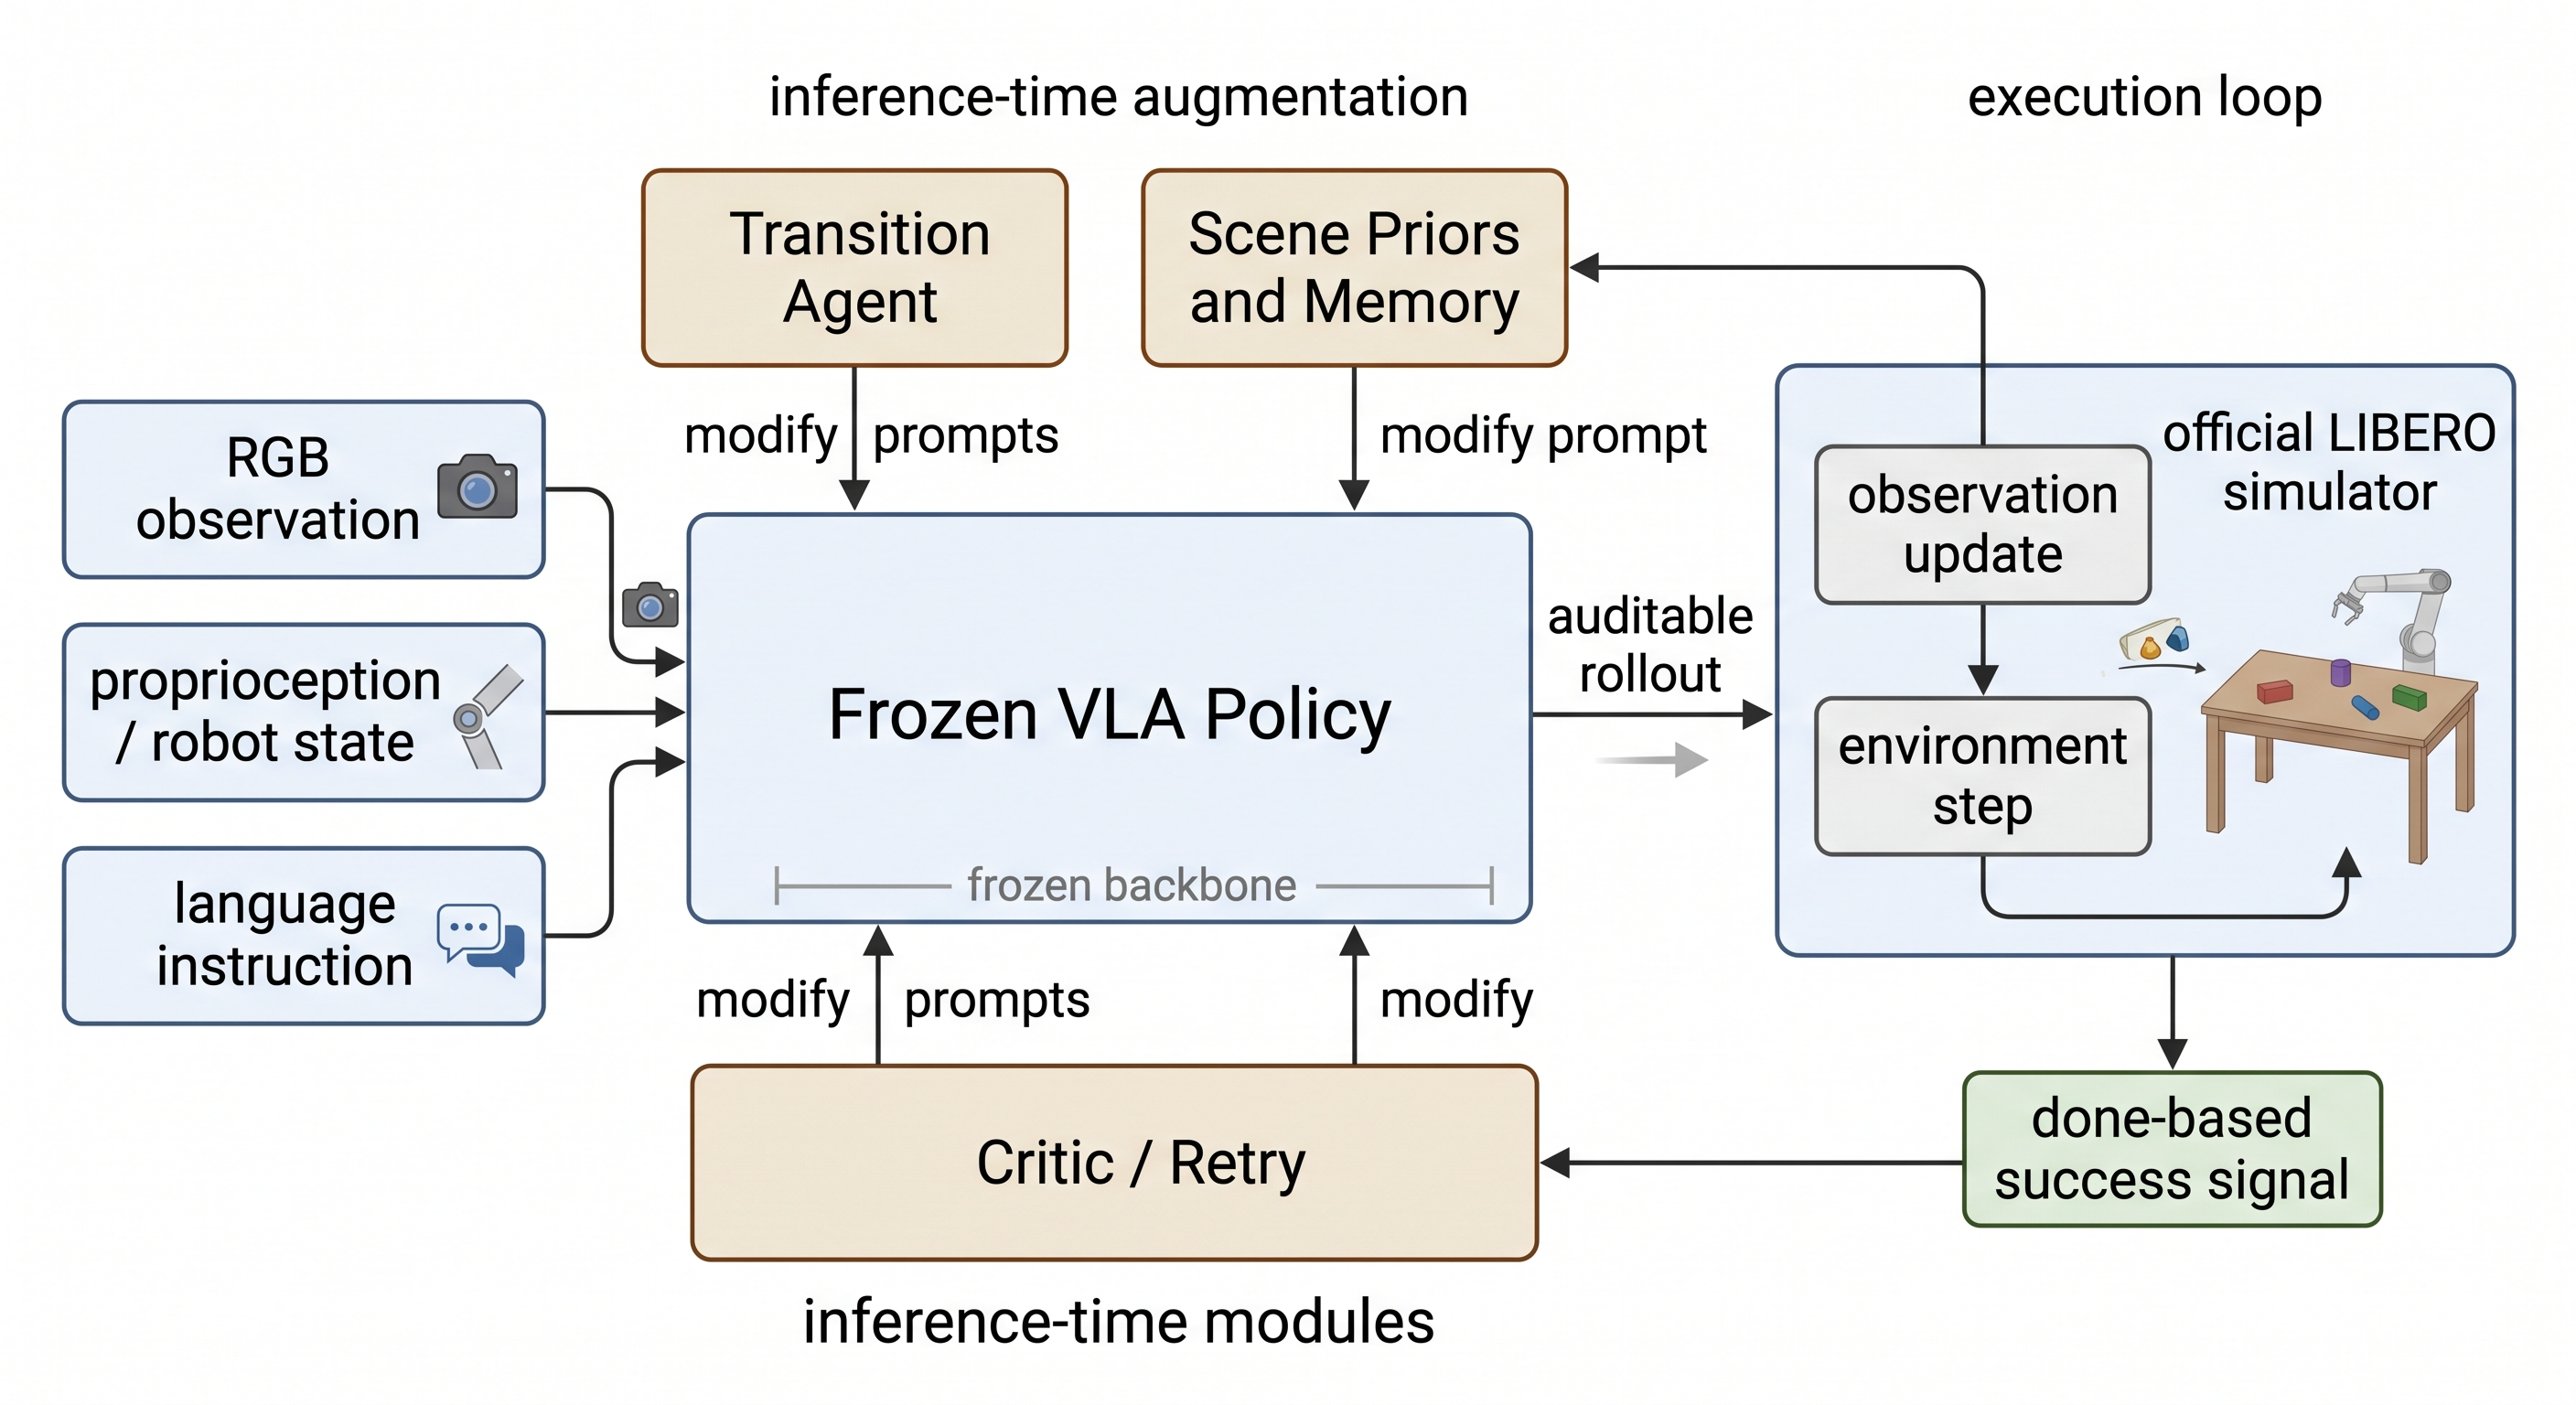
\includegraphics[width=\textwidth]{figures/fig.1-gemini.png}
\caption{Overview of Agentic-VLA. A frozen VLA policy remains the action generator, while Transition, scene priors/memory, and Critic/Retry act as external inference-time process-control modules around an auditable rollout loop in the official LIBERO simulator.}
\label{fig:method_overview}
\end{figure}

\section{Related Work}

\subsection{Foundation VLA Policies and Open Policy Stacks}

Modern VLA research has rapidly progressed from early large-scale visuomotor policies such as RT-1 and RT-2 to more open and generalist families including RoboFlamingo, OpenVLA, Octo, $\pi_0$, and $\pi_{0.5}$ \cite{rt1,rt2,roboflamingo,openvla,octo,pi0,pi05}. In parallel, community infrastructure efforts such as Open X-Embodiment have shifted attention toward shared datasets, open policy stacks, and reproducible evaluation interfaces \cite{openx}. More recent works continue to improve model scale, tokenization, embodiment breadth, or deployment profile, as seen in FAST, Green-VLA, EveryDayVLA, and GR00T \cite{fast,greenvla,everydayvla,gr00t}. This body of work has made frozen or lightly adapted VLAs substantially stronger than earlier policy classes, which makes the remaining long-horizon failures more interesting: the central limitation is often no longer local action generation, but how a strong policy is steered through multi-stage execution.

\subsection{Long-Horizon Benchmarks and Control Bottlenecks}

The long-horizon setting is now supported by a growing benchmark ecosystem. CALVIN and LIBERO established compositional, language-conditioned evaluation suites in which success depends on chaining multiple interaction phases rather than solving a single atomic skill \cite{calvin,libero}. More recent analyses and benchmark efforts, such as Long-VLA and RoboCerebra, further emphasize that temporal consistency, subtask handoff, and recovery from off-nominal states remain major failure sources even when the underlying policy is already capable \cite{longvla,robocerebra}. Our work is motivated directly by this observation. Instead of proposing another policy backbone or another training corpus, we ask whether some of these bottlenecks can be mitigated at inference time through an explicit process-control layer wrapped around a strong frozen LIBERO policy.

\subsection{Agentic Augmentation, Reasoning, and Memory}

Another active direction augments robot control with external reasoning, planning, or structured world interaction. SayCan, PaLM-E, Code as Policies, VoxPoser, and Hi Robot show that language-guided planning, programmatic control, or hierarchical decomposition can improve embodied decision making beyond reactive policy execution alone \cite{saycan,palme,codeaspolicies,voxposer,hirobot}. Recent VLA-centered agentic systems push this idea further. ECoT and Fast ECoT introduce explicit reasoning traces for embodied control \cite{ecot,fastecot}; MemoryVLA studies perceptual-cognitive memory for manipulation \cite{memoryvla}; and ManiAgent, VLA$^2$, and COME illustrate how external modules can be combined with VLA policies to improve robustness or concept coverage \cite{maniagent,vla2,come}. Agentic-VLA is aligned with this trend, but takes a narrower and more auditable stance: our modules remain lightweight, execution-time, and directly attributable to rollout outcomes rather than to a new monolithic planner.

\subsection{Failure Detection, Transition Repair, and Recovery}

Several recent works target the specific question of how to detect and repair failures during execution. Sci-VLA explicitly studies transition insertion for long-horizon state gaps, which is closely related to our motivation for the Transition Agent \cite{scivla}. OneTwoVLA explores adaptive reasoning during action generation \cite{onetwovla}, while FailSafe and Guardian focus on diagnosing planning or execution failures and triggering corrective behavior \cite{failsafe,guardian}. These works collectively suggest that failure handling should be treated as a first-class systems problem rather than as a mere byproduct of better pretraining. Our contribution is complementary: we evaluate a compact stack of transition repair, scene priors with lightweight memory, and critic-triggered retry around a frozen fine-tuned LIBERO policy, and we report its value using auditable rollout evidence instead of proxy judgments.

\section{Agentic-VLA Framework}

\subsection{Frozen Policy and Chunked Execution}

Our baseline is a fine-tuned \texttt{pi05\_libero} policy derived from the $\pi_{0.5}$ family and served through the official OpenPI policy stack \cite{pi05,pi0}. Given the current visual observations, proprioceptive state, and task prompt, the policy predicts an action chunk that is executed for a fixed number of steps before replanning. This action-chunk execution scheme is effective for many short- and medium-horizon manipulation tasks. However, as also observed by recent long-horizon VLA work \cite{longvla,scivla}, it can fail when locally plausible chunks do not smoothly connect successive subtask states. Agentic-VLA is designed to repair this failure pattern without changing the action generator itself: the backbone remains frozen, while a small external loop intervenes only when rollout evidence suggests that additional process control is beneficial.

\subsection{Transition Agent}

The Transition Agent targets \emph{state-gap} failures between adjacent subtask phases. Motivated by recent observations that long-horizon VLA rollouts often fail at subtask boundaries rather than within well-practiced atomic skills \cite{scivla,longvla}, it monitors recent end-effector motion and detects stalled progress when the average displacement over a sliding window falls below a threshold. Once triggered, the module temporarily overrides the nominal prompt with a transition prompt that requests a safe neutral motion and a reconnection maneuver. The VLA then generates a short intermediate action sequence aimed at moving the robot to a more controllable state before normal execution resumes. The backbone remains frozen, and the intervention is implemented entirely at the prompt and execution levels. Figure~\ref{fig:transition_gap} visualizes the intended repair mechanism.

\begin{figure}[t]
\centering
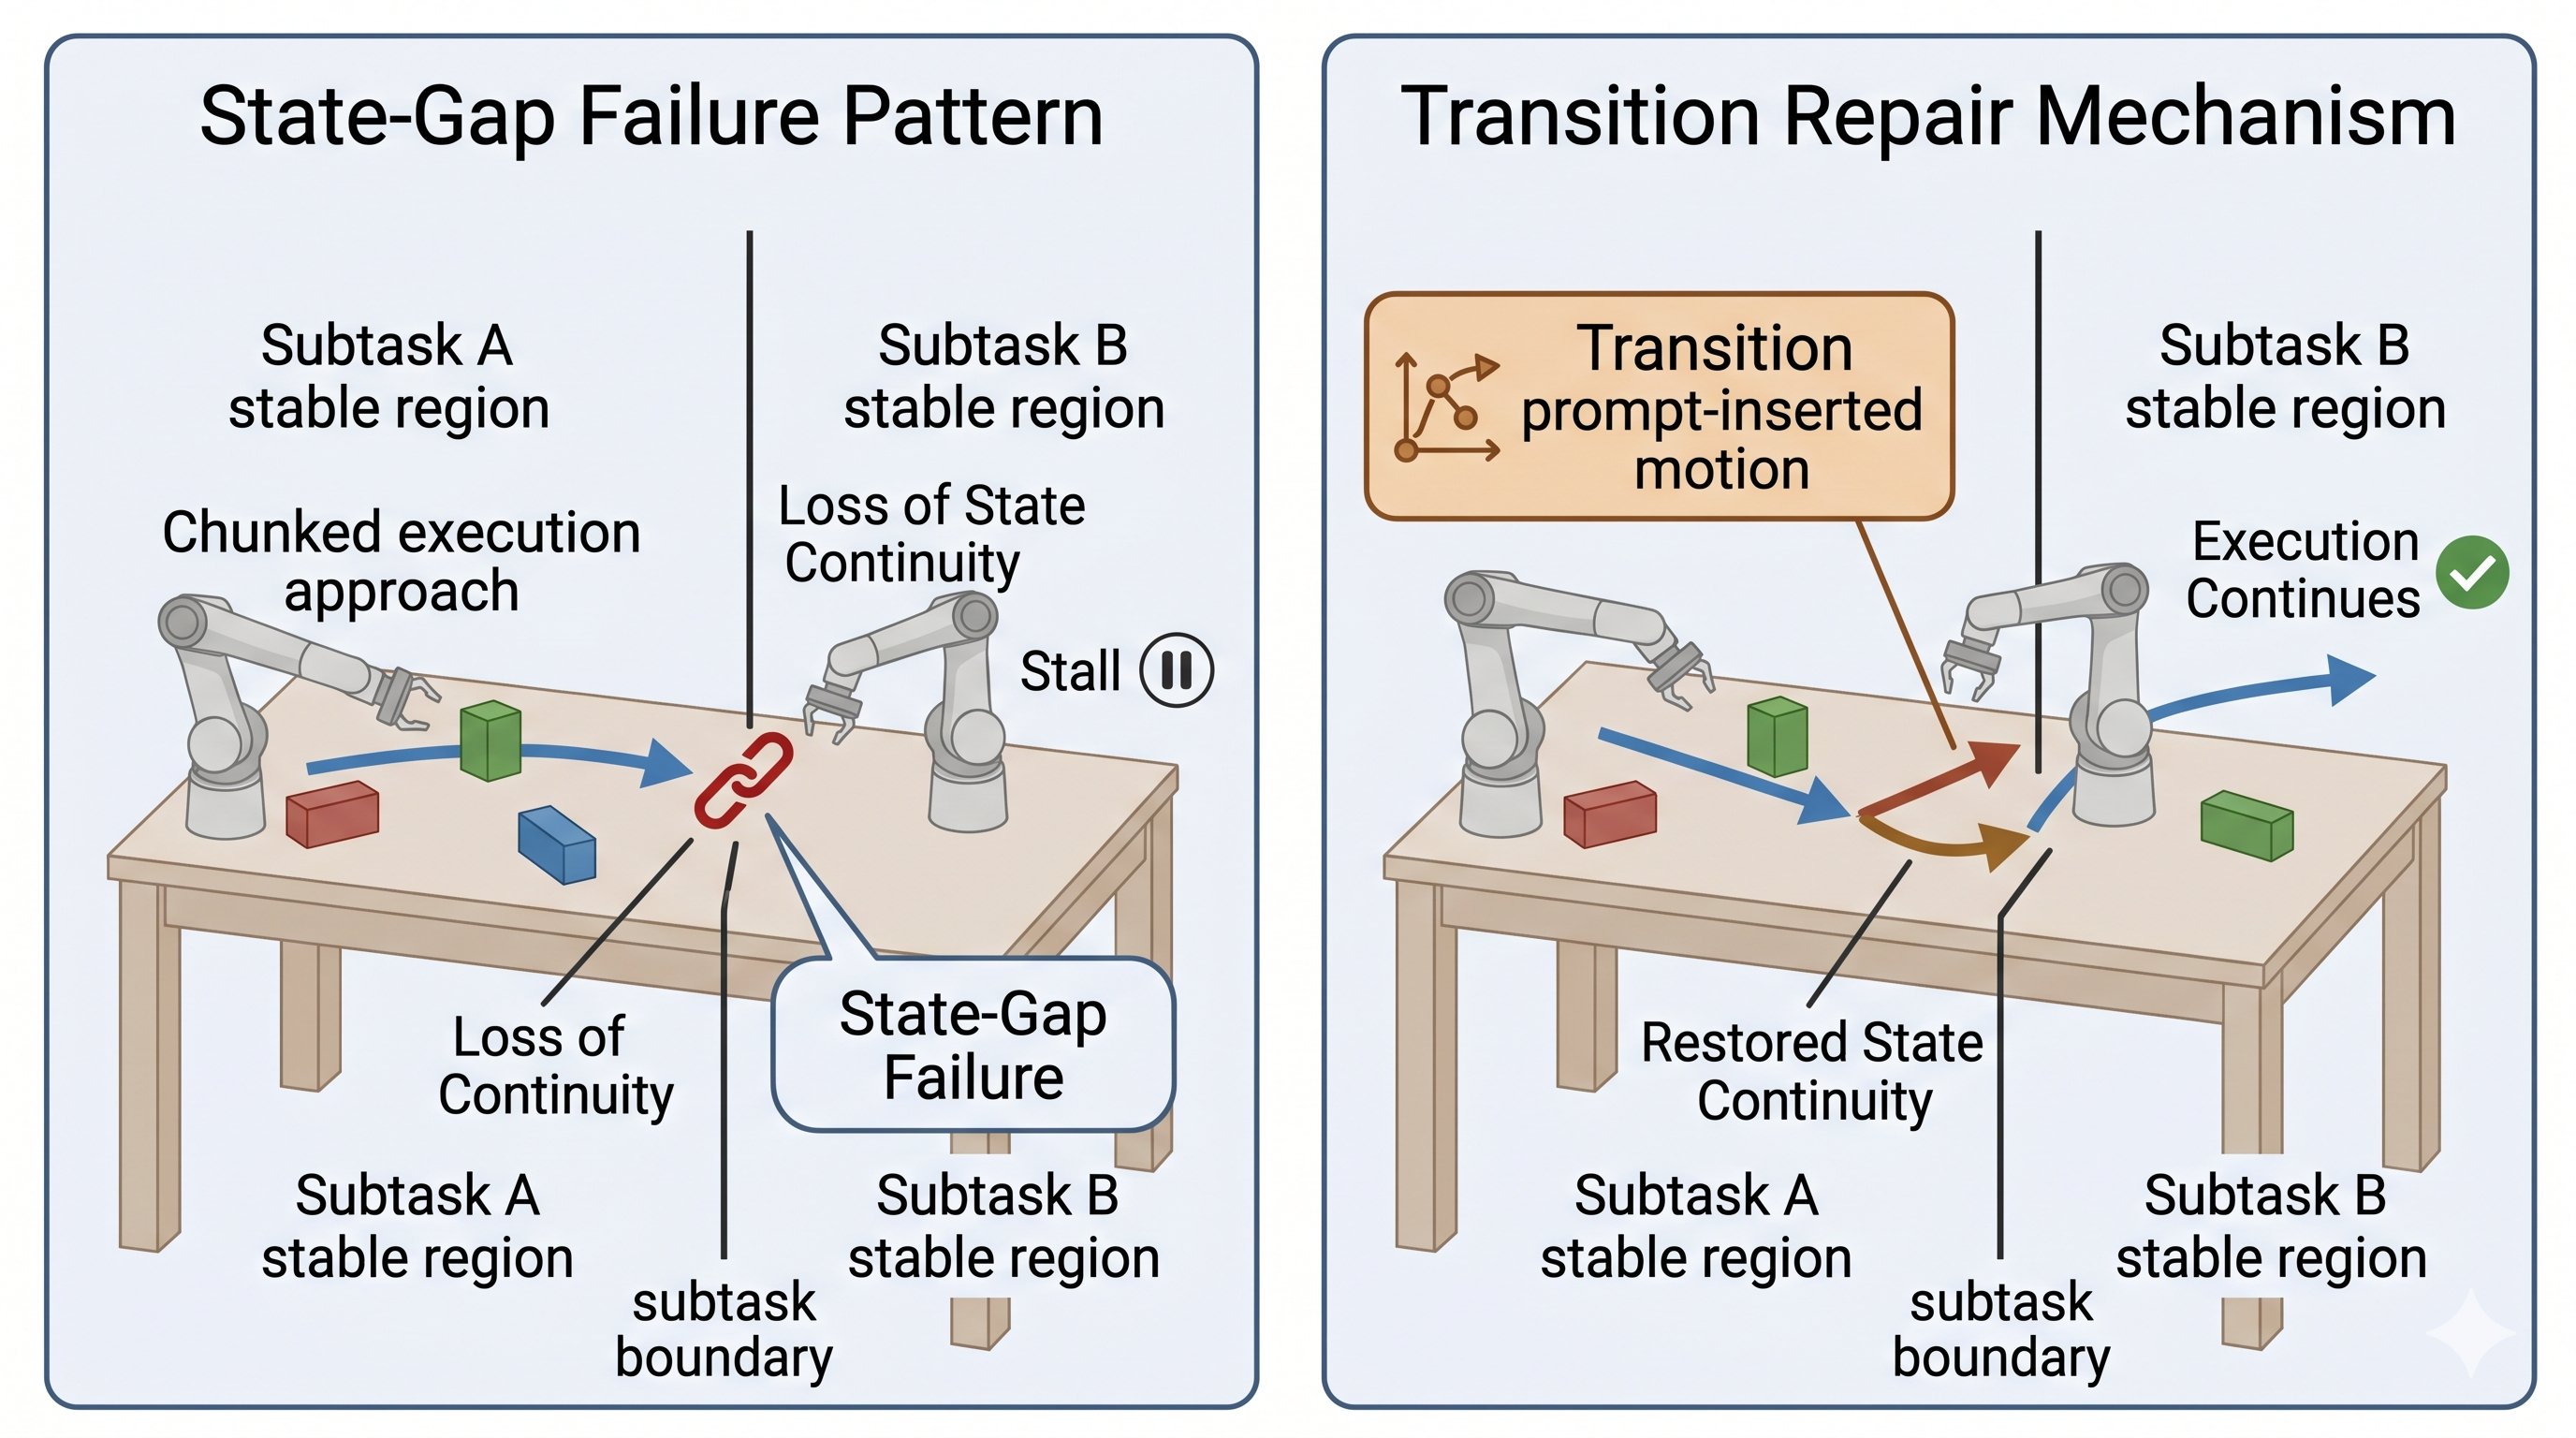
\includegraphics[width=\textwidth]{figures/fig.2-gemini.png}
\caption{Mechanism schematic of the Transition Agent. Left: chunked execution reaches a subtask boundary and loses state continuity. Right: the Transition Agent inserts an intermediate reconnection motion so that normal policy execution can resume from a more controllable state.}
\label{fig:transition_gap}
\end{figure}

\subsection{Scene Priors and Memory}

The scene-prior and memory module injects lightweight structured hints based on task-relevant entities, such as suggested vertical offsets, gripping strength, or approach direction for specific objects. This component is motivated by works showing that structured reasoning, memory, or external grounding can improve VLA robustness \cite{ecot,memoryvla,vla2}. In our implementation, the module remains deliberately simple and interpretable: instead of retrieving large document collections or training a separate memory policy, it augments the prompt with topology-aware priors extracted from object and scene keywords and records simple episodic cues from successful executions. Its purpose is to reduce avoidable ambiguity at execution time and bias the frozen policy toward more stable interaction patterns. Figure~\ref{fig:scene_priors_memory} summarizes the design.

\begin{figure}[t]
\centering
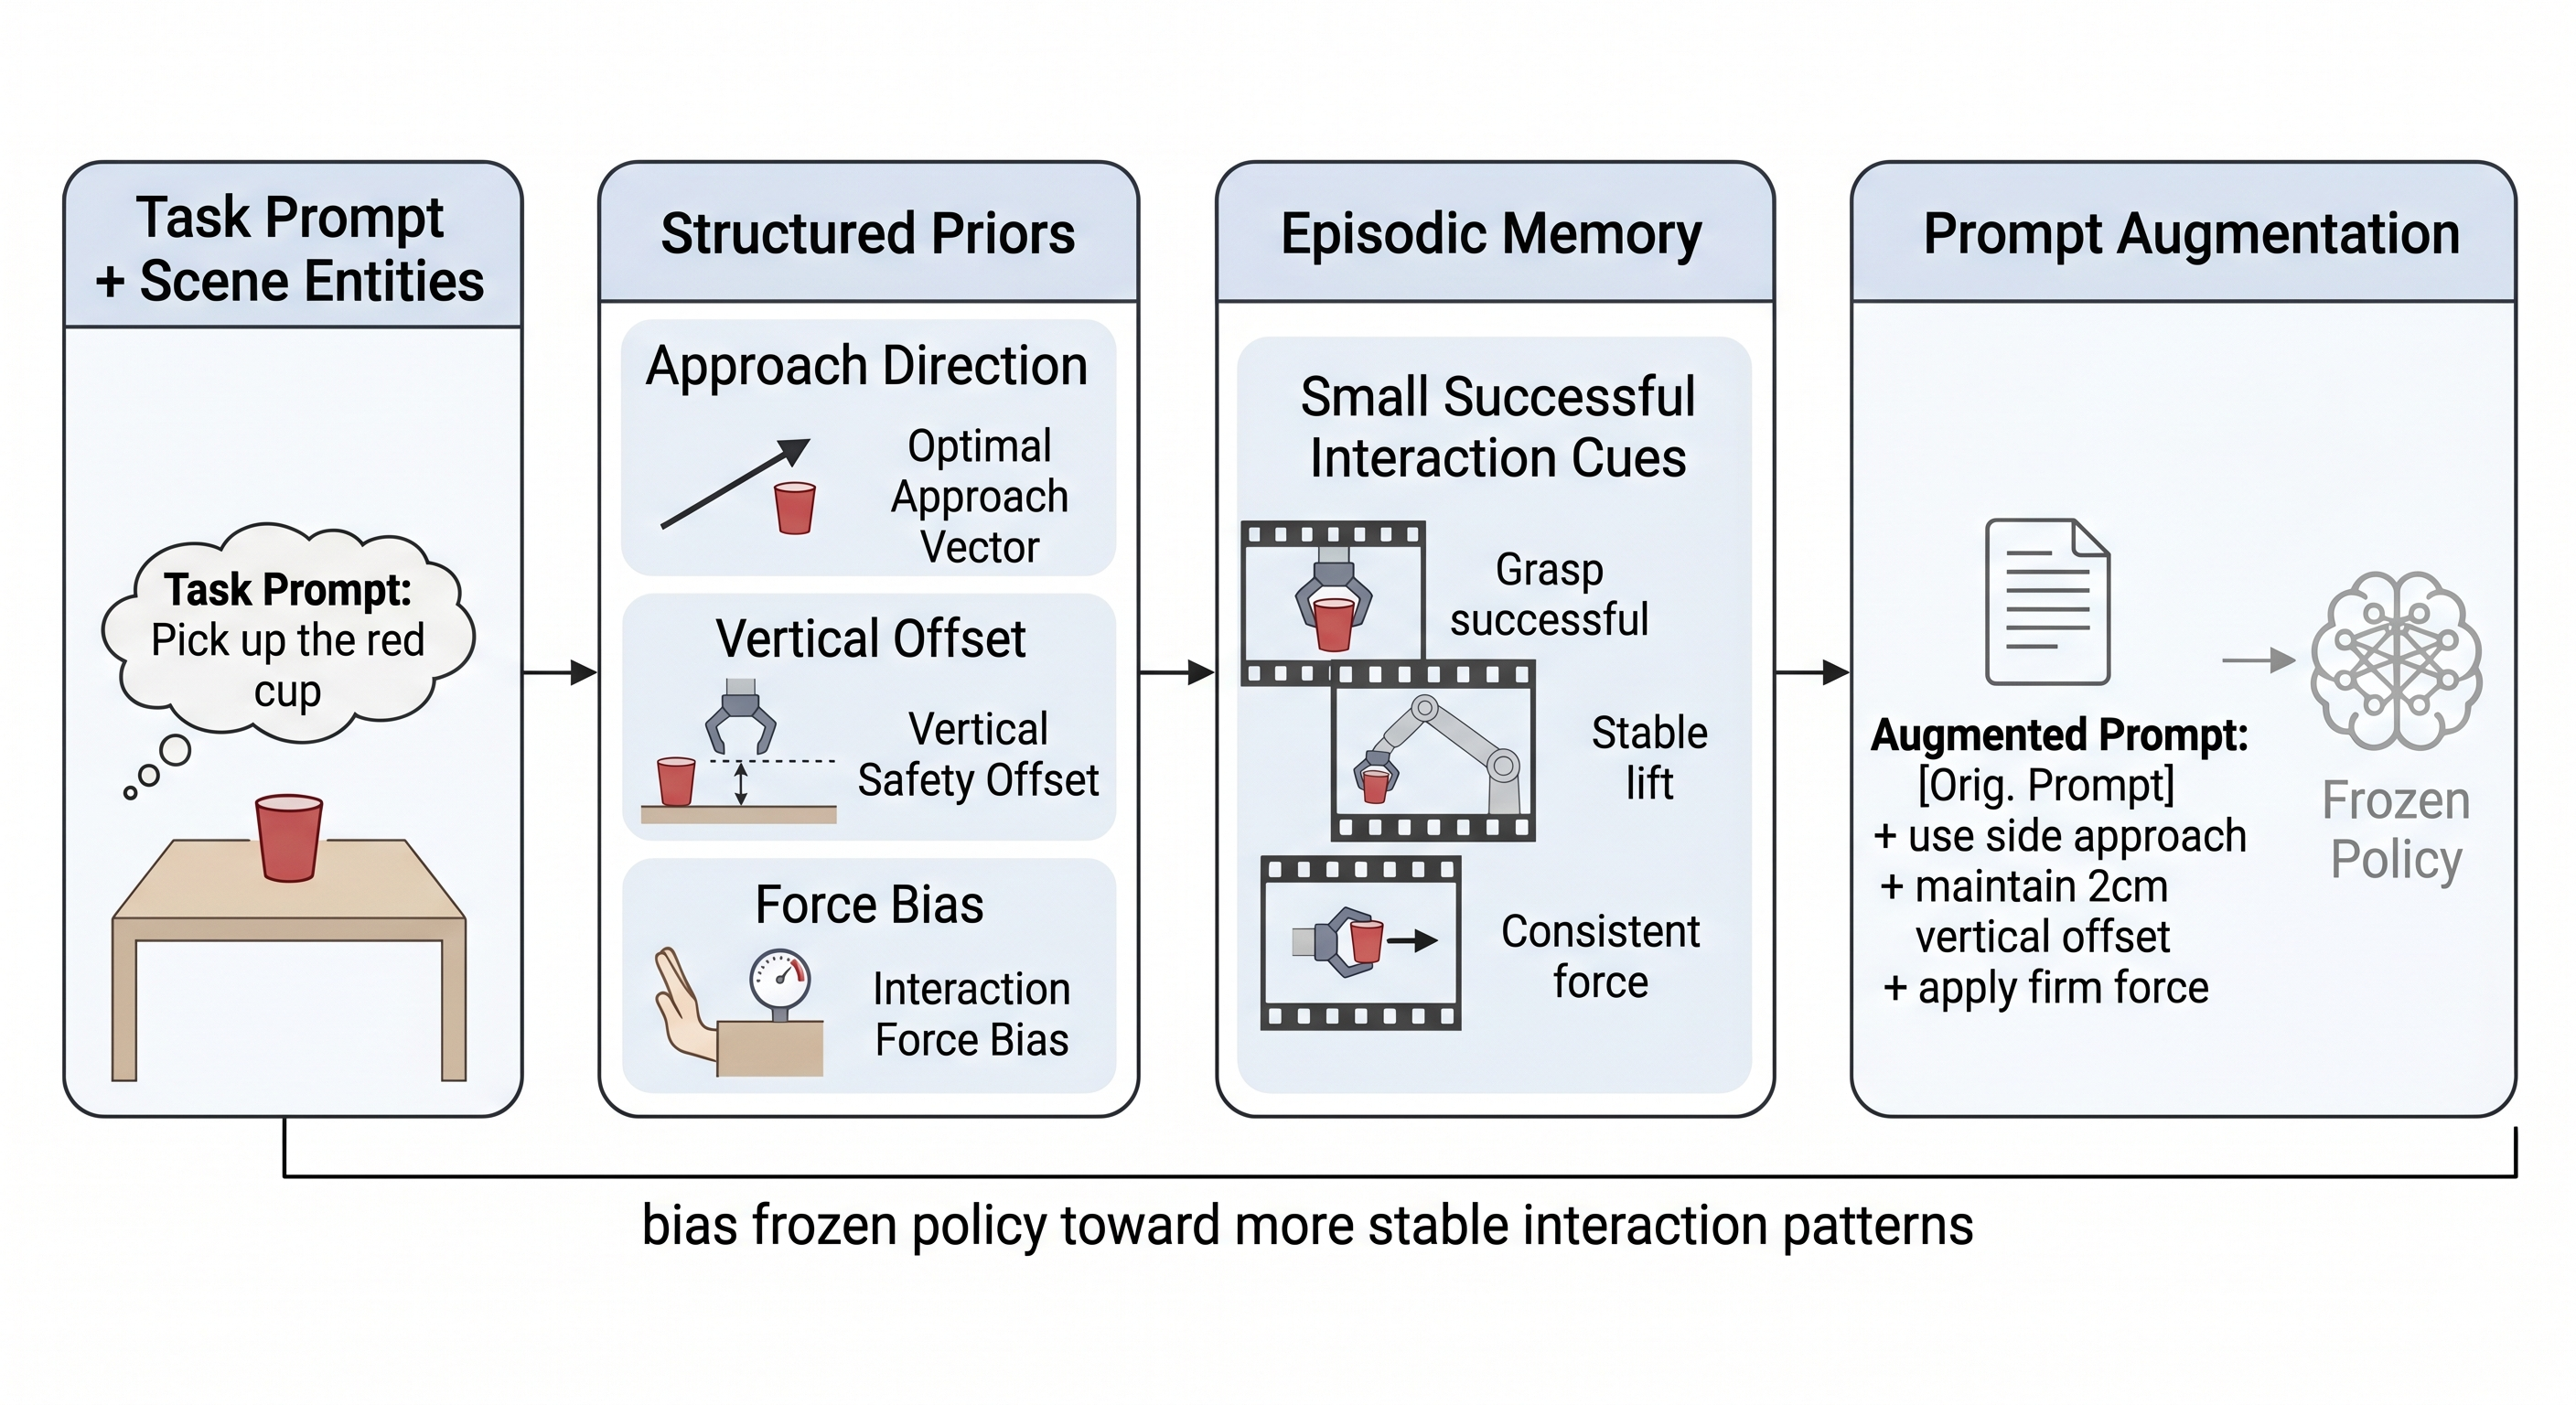
\includegraphics[width=\textwidth]{figures/fig.3-gemini.png}
\caption{Scene priors and memory in Agentic-VLA. Lightweight task entities are converted into structured priors and episodic cues, which are then injected into the prompt to bias the frozen policy toward more stable interaction patterns.}
\label{fig:scene_priors_memory}
\end{figure}

\subsection{Critic and Retry}

The Critic/Retry module periodically evaluates the current execution state and determines whether the policy appears stuck, incomplete, or inconsistent with the task objective. The design is informed by recent work on failure diagnosis, recovery, and reflective embodied reasoning \cite{failsafe,guardian,onetwovla}. When a likely failure pattern is detected, the module first triggers a recovery prompt intended to return the robot to a safer operating state, then issues a retry prompt tailored to the inferred error type. Operationally, this clears the current action plan and allows the policy to re-enter the rollout from a more favorable state. Within the full system, the module is intended to convert locally recoverable failures into successful episodes rather than merely label success or failure.

\begin{figure}[t]
\centering
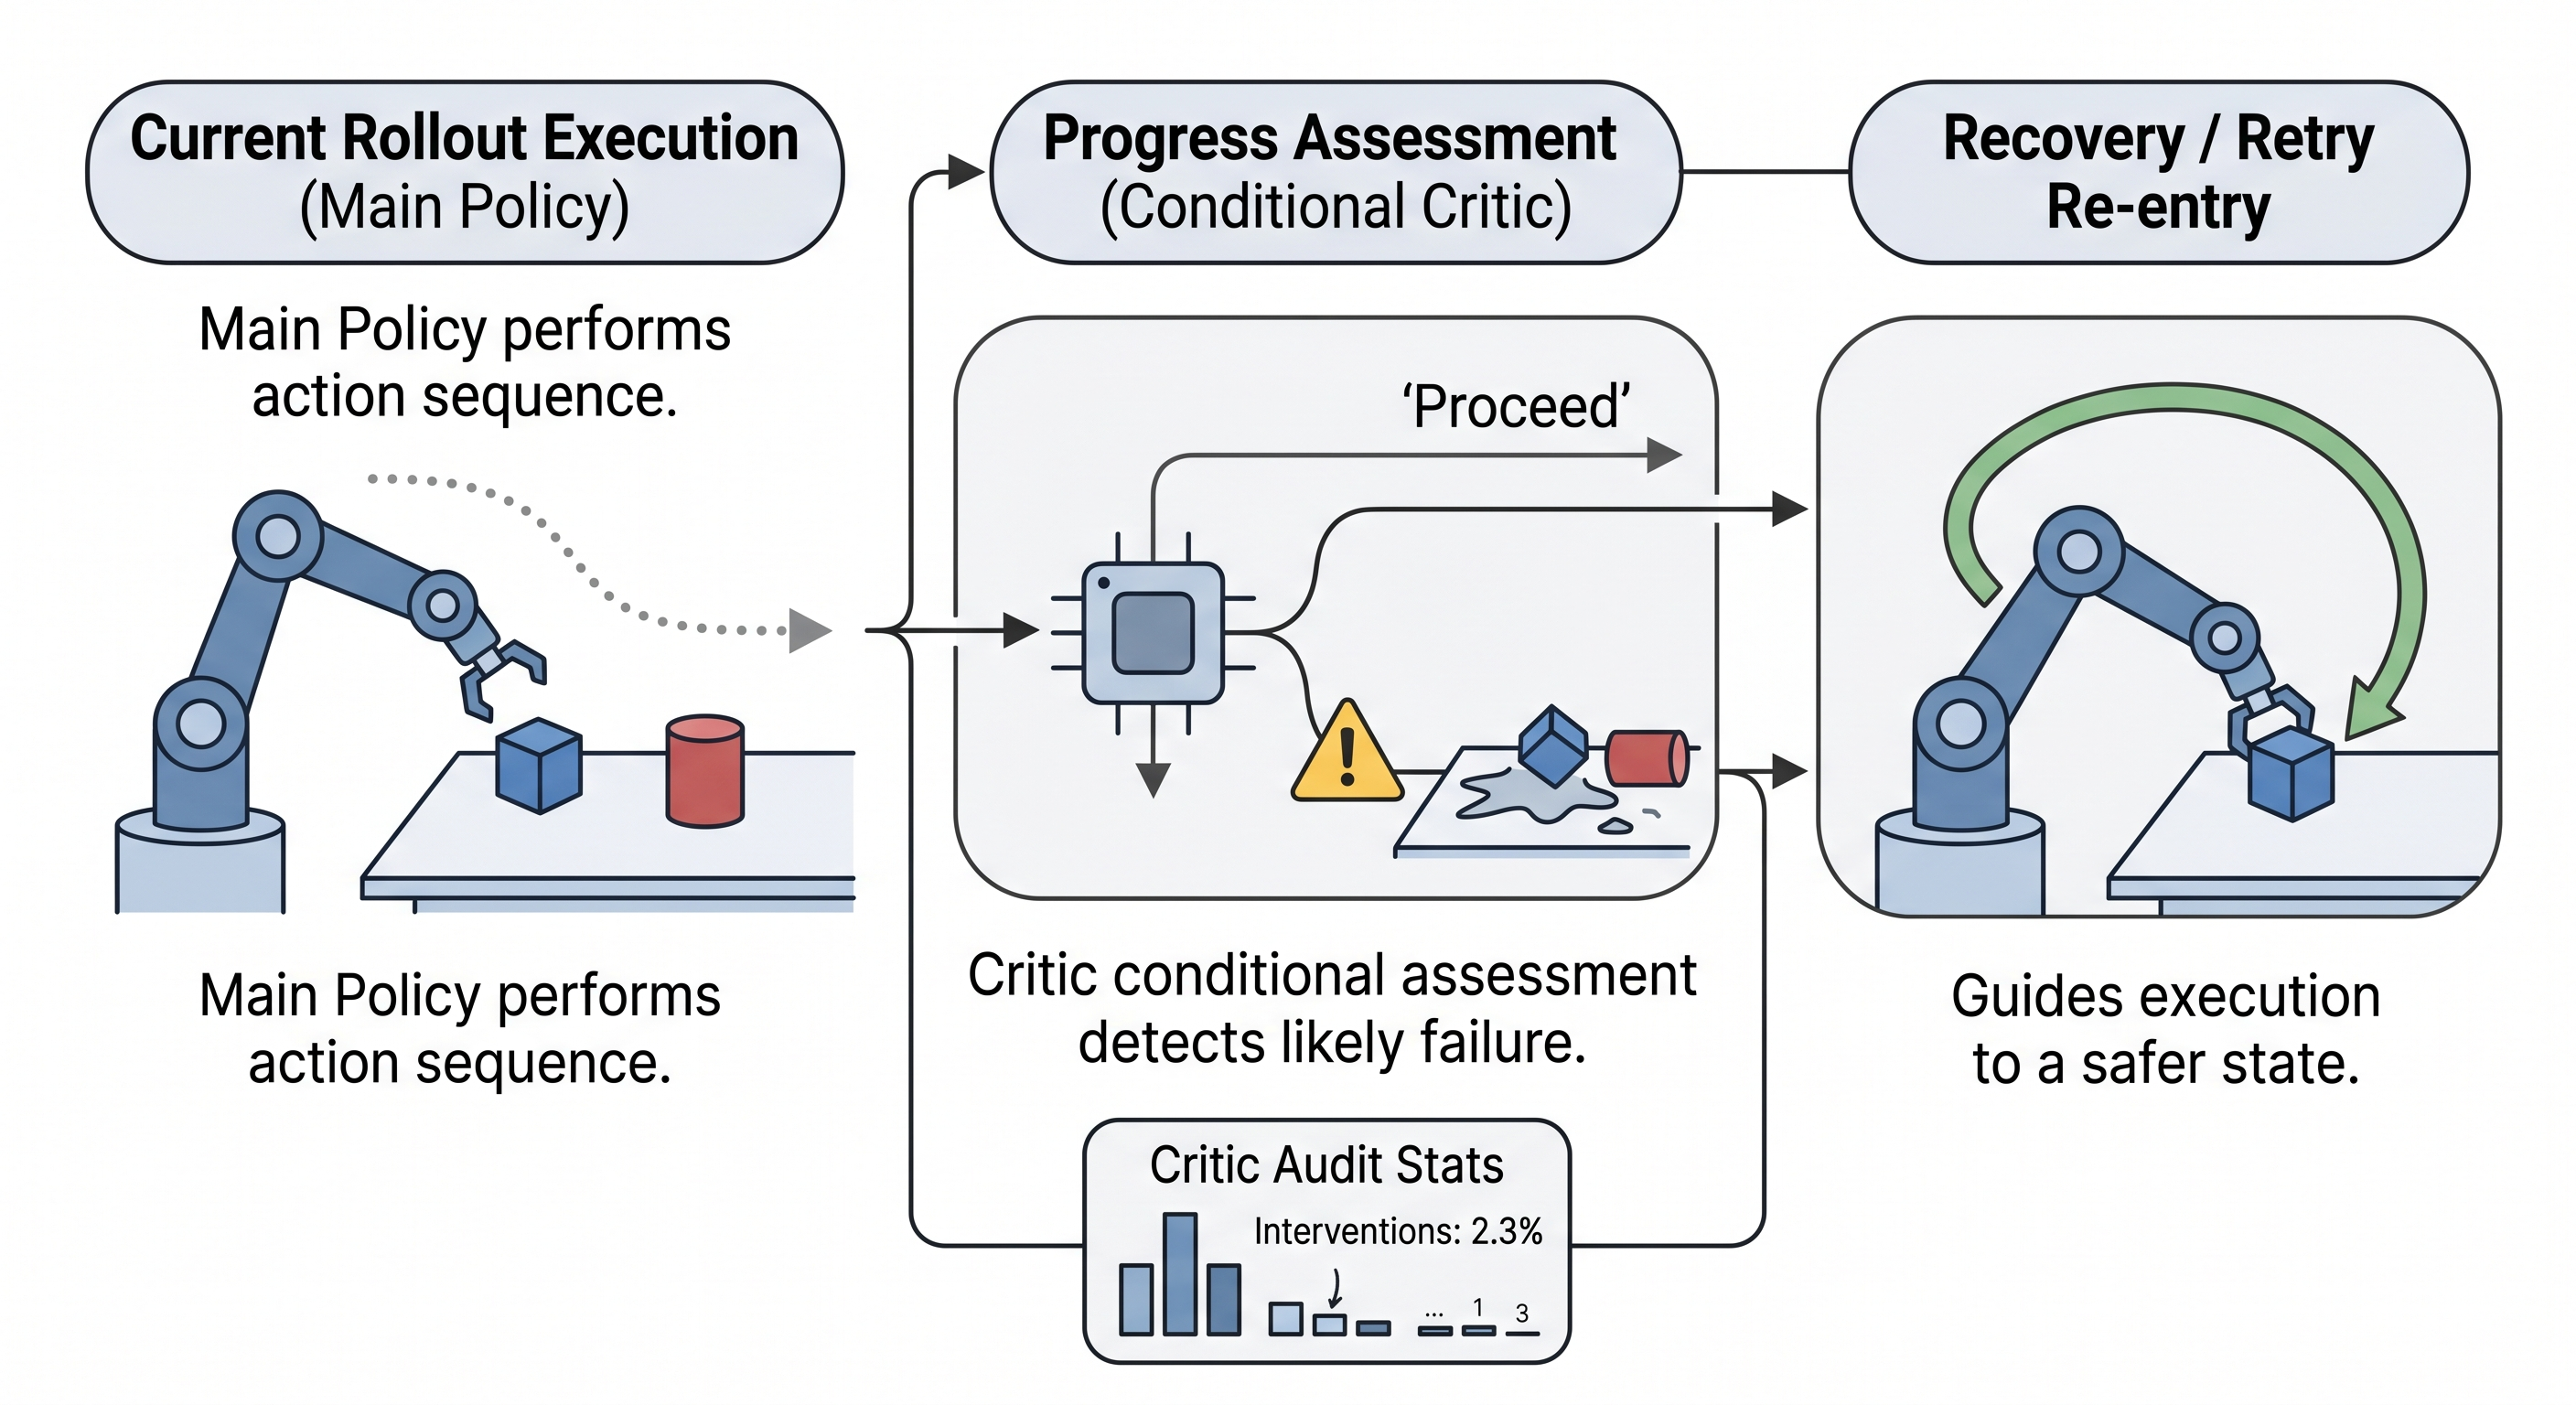
\includegraphics[width=\textwidth]{figures/fig.4-gemini.png}
\caption{Critic/Retry in Agentic-VLA. A conditional critic monitors rollout progress, detects likely execution inconsistency, and guides recovery or retry re-entry only when intervention is needed, keeping the base policy as the primary controller.}
\label{fig:critic_retry_flow}
\end{figure}

\subsection{Unified Agentic Execution Loop}

The final Agentic-VLA framework wraps these modules around the baseline VLA policy. Conceptually, the system spans a spectrum from unmodified \texttt{pi05\_libero} to the complete agentic configuration (\textbf{Full}), with individual modules remaining independently switchable for engineering control and audit. Figure~\ref{fig:method_overview} provides the system-level view, while Figures~\ref{fig:transition_gap} and~\ref{fig:critic_retry_flow} isolate the two main intervention mechanisms. In the experiments, the primary quantitative comparison is the head-to-head evaluation between \texttt{pi05\_libero} and the complete Agentic-VLA system on \texttt{libero\_10}; intermediate variants are retained as supporting evidence for mechanism analysis.

\subsection{Scope Relative to the Current Codebase}

The current project codebase continues to evolve beyond the configuration quantitatively analyzed in this paper. In particular, the repository already contains ongoing extensions toward structured on-demand planning, explicit router-expert-verifier orchestration, and a more formalized agent-level mixture-of-experts loop. These components are engineering continuations of the same process-control direction, but they are \emph{not} part of the quantitative claims made here because they do not yet have completed suite-level rollout evidence under the same evaluation protocol. This paper therefore reports only the validated configuration centered on Transition, scene priors/memory, and Critic/Retry around a frozen \texttt{pi05\_libero} backbone.

\subsection{Design Rationale}

The framework is designed as a \emph{minimal external augmentation} rather than a new monolithic controller. This choice has three advantages. First, it preserves the capabilities of the strong baseline VLA and makes improvement attributable to explicit interventions rather than confounding architecture changes. Second, it keeps deployment practical because modules can be enabled or disabled independently under different latency or memory budgets. Third, it yields a clearer scientific question: if long-horizon failures largely arise from process-control gaps, then targeted transition and recovery interventions should matter most on weak tasks, while simpler in-domain tasks should remain largely unaffected.

\subsection{Target Failure Modes}

Agentic-VLA is designed around a concrete failure taxonomy rather than a generic ``reasoning helps'' claim. We distinguish four recurring failure modes in long-horizon LIBERO rollouts: \emph{transition failures}, \emph{contact or grasp failures}, \emph{completion failures}, and \emph{recovery failures}. The Transition Agent mainly targets the first class, the scene-prior and memory module mainly addresses the second and third through structured hints, and the Critic/Retry module addresses the fourth through diagnosis and rollback-like re-entry. This mapping matters for interpretation: if a module improves performance, we should also observe changes in the corresponding failure pattern.

\section{Experiments}

\subsection{Experimental Setup}

We evaluate in the official LIBERO simulator through interactive rollouts \cite{libero}. The main quantitative comparison is the completed head-to-head evaluation on \texttt{libero\_10}, which most clearly exposes the long-horizon weaknesses of the baseline policy and is the only suite for which the main comparison is complete. Each policy is evaluated for 20 trials on each of the 10 tasks, for a total of 200 episodes per method in the completed main comparison.

\subsection{Task Suite, Baseline, and Metrics}

The baseline policy is \texttt{pi05\_libero}. We report task success rate as the main metric and additionally log transition counts, retry counts, recovery-to-success statistics, and average episode length for agentic variants. These measurements separate raw task completion from the mechanism by which improvement occurs.

\subsection{Submission Scope}
The study is centered on \texttt{libero\_10}. Within this suite, the primary comparison is between \texttt{pi05\_libero} and Full Agentic-VLA. This suite retains visible headroom over the baseline and exposes the long-horizon failure modes that are most relevant to our setting. Intermediate module variants are used as supporting evidence for mechanism analysis rather than as the main quantitative comparison.

\subsection{Evidence Hierarchy and Claim Boundary}

We intentionally separate three evidence tiers. The first tier is the \emph{completed main comparison}: the baseline and refined Full Agentic-VLA head-to-head evaluation on \texttt{libero\_10}. The second tier is \emph{supporting diagnosis}: targeted follow-up runs on the exposed weak-task subset (T6/T8/T9) and the corresponding minimal ablations used to interpret module interaction. The third tier is \emph{ongoing system extension}: newer planner-centric and router-centric code paths that are present in the repository but are not yet backed by completed suite-level rollouts under the same protocol. All quantitative claims in this paper are restricted to the first two tiers.

\subsection{Reproducibility and Logging}

Each run produces structured per-run records together with per-task metrics, intervention statistics, and rollout videos. We additionally preserve checkpointed progress for long benchmark runs so that completed tasks are not silently discarded during continuation. This logging design keeps every reported number traceable to rollout evidence rather than manual note-taking or partial console logs. The final analysis uses only the completed result directory of the refined Full run on \texttt{libero\_10} (20 trials per task) together with the corresponding verified baseline run on the same suite; incomplete or pilot runs are excluded from the quantitative tables.

\subsection{Real Rollout Protocol}

All reported results come from \emph{interactive rollouts} in the official LIBERO simulator rather than offline scoring, proxy metrics, or mock evaluation. The policy is served through the official OpenPI stack, and success is determined by the environment's task completion signal during environment stepping. For each episode, we also save structured local records and rollout videos. The resulting protocol evaluates embodied execution directly while remaining distinct from physical-robot experiments: LIBERO provides real rollouts in simulation, not real-world hardware trials.

\subsection{Implementation Details}

The baseline controller uses the \texttt{pi05\_libero} policy through the official OpenPI stack. The evaluated full system combines Transition, scene priors/memory, and Critic/Retry in a unified inference-time loop. Follow-up diagnosis on the exposed weak-task region leads to three control-side refinements: structured merging between manipulated-object priors and target-region priors, task-aware transition and recovery prompts for difficult placement regimes such as stove and microwave tasks, and more conservative task-specific thresholds for intervention timing. These changes modify execution control rather than the backbone itself and are introduced to repair exposed weak-task failures rather than to claim uniform improvement across \texttt{libero\_10}. For the critic component, we use a locally verified Qwen3-VL checkpoint loaded through the Hugging Face \texttt{transformers} stack with \texttt{bitsandbytes} quantization. The current deployment uses 4-bit NF4 quantization with double quantization enabled, \texttt{bfloat16} compute dtype, and automatic device placement so that the full critic module fits within a single RTX 4090 budget. Newer planner-side protocol extensions in the repository reuse the same base infrastructure but are excluded from the quantitative analysis here.

\subsection{Main Results}

The verified baseline reaches 90.0\% (180/200) on the official \texttt{libero\_10} suite, indicating that the underlying frozen policy is already strong. The remaining errors are concentrated on a small set of long-horizon composite tasks, most notably Task 8 at 55.0\%. This pattern is consistent with recent VLA literature: stronger backbones improve local competence, but long-horizon robustness remains the dominant bottleneck \cite{longvla,onetwovla,scivla}.

Against this baseline, the completed refined Full Agentic-VLA run reaches 92.5\% (185/200) under official rollout evaluation. The gain is driven primarily by repairing the weak-task region (Task 8: 55.0\% $\rightarrow$ 75.0\%), while maintaining near-saturation on most tasks. At the same time, the per-task view reveals small fluctuations on a subset of non-weak tasks, which cautions against overclaiming uniform improvement across the entire suite.

The main run therefore supports a restrained interpretation. Agentic-VLA is useful as a deployment-time process-control layer, but its benefit is task-dependent and its hardest failures are repaired only after targeted control-side refinements. Mechanism statistics reinforce the same conclusion. In the audited earlier full-stack run, transition interventions are frequent and often associated with successful episodes, whereas critic-triggered retries remain absent in the tuned configuration. The resulting picture is not one of a universally beneficial stack, but of a practical control layer whose gains depend on where the rollout failure mode lies.

\begin{table}[t]
\caption{Main completed comparison on \texttt{libero\_10}. Both methods are evaluated through official LIBERO interactive rollouts with 20 trials per task.}
\label{tab:main_libero10_results}
\centering
\begin{tabular}{lcc}
\toprule
Method & Success (\%) & Episodes \\
\midrule
\texttt{pi05\_libero} & 90.0 & 180/200 \\
Refined Full Agentic-VLA & \textbf{92.5} & \textbf{185/200} \\
\bottomrule
\end{tabular}
\end{table}

\begin{table}[t]
\caption{Per-task results on \texttt{libero\_10}. The completed refined Full run shows a structured pattern rather than uniform improvement: the dominant weak-task failure (Task 8) is repaired while most tasks remain near saturation, but small task-dependent fluctuations persist.}
\label{tab:libero10_task_results}
\centering
\begin{tabular}{lcccccccccc}
\toprule
Method & T0 & T1 & T2 & T3 & T4 & T5 & T6 & T7 & T8 & T9 \\
\midrule
\texttt{pi05\_libero} & 90.0 & 100.0 & 95.0 & 90.0 & 100.0 & 95.0 & 80.0 & 100.0 & 55.0 & 95.0 \\
Refined Full & \textbf{95.0} & 100.0 & 90.0 & \textbf{95.0} & 95.0 & \textbf{100.0} & 80.0 & 100.0 & \textbf{75.0} & 95.0 \\
\bottomrule
\end{tabular}
\end{table}

\subsection{Per-Task and Mechanism Analysis}

The weak-task subset is the most informative regime for analyzing process control because failure modes that matter there are largely invisible on saturated tasks. As shown in Table~\ref{tab:libero10_task_results}, the completed refined Full run is not a simple weak-task-repair story. Refined Full improves several baseline-imperfect tasks (T0, T2, T3, and T5), preserves parity on saturated tasks (T1, T4, and T7), and matches the baseline on T6, while still leaving T8 as the dominant residual weak point. This structure is more naturally read as uneven control benefit than as a uniform suite-wide shift, which is consistent with recent analyses that emphasize subtask coupling and accumulated execution drift rather than average performance alone \cite{longvla,robocerebra,guardian}.

Targeted diagnosis on the exposed weak-task regime sharpens this picture. After the earlier full-stack run exposed the weak region around T6/T8/T9, a task-targeted v2 follow-up reaches 70.0\% on Task 8, 100.0\% on Task 9, and 90.0\% on Task 6. Table~\ref{tab:targeted_followup_results} summarizes these results together with the corresponding earlier full-stack values. The follow-up is therefore best interpreted as a targeted repair of exposed failure modes, not as evidence of universal improvement across the suite. Task 8 is particularly informative: removing scene priors and memory drops performance from 70.0\% to 60.0\%, indicating a positive contribution from that module group, whereas removing the critic leaves the result unchanged at 70.0\%. Most notably, removing transition raises Task 8 to 80.0\%, revealing that the remaining limitation lies less in the absence of useful modules than in imperfect coordination among them.

Intervention statistics support the same reading. In the audited earlier full-stack run, the system averages 0.81 transition interventions per episode, and transitions are associated with success in 88.9\% of the episodes where they are used. By contrast, critic-triggered retries are never activated in the tuned configuration. The current evidence therefore points to a partially effective process-control layer: explicit transition handling and scene priors/memory can help on difficult cases, whereas Critic/Retry remains under-activated and the interaction policy still leaves room for further engineering \cite{failsafe,guardian}.

\subsection{Discussion of Current Limits}

The current evidence should be interpreted conservatively. First, the completed main comparison demonstrates a real gain over a strong baseline, but the gain remains modest at the suite level because the baseline is already strong and most tasks are near saturation. Second, the weak-task diagnosis shows that modules can interfere with one another even when each of them is individually motivated; the central remaining bottleneck is now coordination rather than the absence of process control altogether. Third, the present critic is better understood as an audit and trigger component than as a mature recovery controller, since retry behavior remains largely dormant in the tuned setting. Finally, ongoing planner-centric extensions in the codebase are promising for future versions of Agentic-VLA, but they must be validated by completed rollout evidence before being folded into the paper's quantitative story.

\begin{table}[t]
\caption{Targeted diagnosis on the weak-task subset. ``Original Full'' denotes the earlier full-stack configuration that exposed the weak-task failures, while ``Task-targeted v2'' denotes the follow-up configuration evaluated only on T6/T8/T9 after diagnosis.}
\label{tab:targeted_followup_results}
\centering
\small
\begin{tabular}{lccc}
\toprule
Method & T6 & T8 & T9 \\
\midrule
\texttt{pi05\_libero} & 80.0 & 55.0 & 95.0 \\
Original Full & 80.0 & 40.0 & 90.0 \\
Task-targeted v2 & 90.0 & 70.0 & 100.0 \\
Transition only & \textbf{100.0} & \textbf{80.0} & 90.0 \\
Graph+Memory only & 80.0 & 60.0 & \textbf{100.0} \\
Critic only & 90.0 & 70.0 & 90.0 \\
\bottomrule
\end{tabular}
\end{table}

\section{Conclusion}

We present Agentic-VLA, a modular inference-time augmentation framework for long-horizon VLA execution. The central premise is that many failures of strong fine-tuned VLA policies arise not from missing atomic skills, but from missing process control across transitions, failures, and recoveries. The completed \texttt{libero\_10} study supports this premise in a conservative form: explicit execution-time augmentation improves a strong frozen \texttt{pi05\_libero} baseline from 90.0\% to 92.5\% under official rollout evaluation in the LIBERO simulator, with the dominant weak task improving from 55.0\% to 75.0\%. The weak-task diagnosis further clarifies where that effect comes from and where it does not. Structured prior merging and task-aware transition/recovery refinement improve the exposed weak-task regime, scene priors and memory contribute positively on difficult cases, the critic remains under-activated, and the dominant remaining challenge is no longer whether process control matters, but how to coordinate multiple control modules without introducing avoidable interference. More broadly, these results suggest that once strong VLA backbones are available, explicit execution-time process control is a practical and scientifically informative direction for embodied intelligence. Current ongoing extensions, including structured on-demand planning and explicit router-expert-verifier orchestration, are promising but remain outside the quantitative claims of this paper until they are validated by completed rollout evidence.

\begin{thebibliography}{31}
\bibitem{rt1}
Brohan, A., Brown, N., Carbajal, J., et al.: RT-1: Robotics Transformer for Real-World Control at Scale. arXiv preprint arXiv:2212.06817 (2022)

\bibitem{rt2}
Brohan, A., Brown, N., Carbajal, J., et al.: RT-2: Vision-Language-Action Models Transfer Web Knowledge to Robotic Control. In: Conference on Robot Learning (2023)

\bibitem{palme}
Driess, D., Xia, F., Sajjadi, M.S.M., et al.: PaLM-E: An Embodied Multimodal Language Model. In: International Conference on Machine Learning (2024)

\bibitem{saycan}
Ahn, M., Brohan, A., Brown, N., et al.: Do As I Can, Not As I Say: Grounding Language in Robotic Affordances. In: Conference on Robot Learning (2022)

\bibitem{codeaspolicies}
Liang, J., Huang, W., Zeng, A., et al.: Code as Policies: Language Model Programs for Embodied Control. In: IEEE International Conference on Robotics and Automation (2023)

\bibitem{voxposer}
Huang, W., Abbeel, P., Pathak, D., et al.: VoxPoser: Composable 3D Value Maps for Robotic Manipulation with Language Models. In: Conference on Robot Learning (2023)

\bibitem{openx}
Open X-Embodiment Collaboration: Open X-Embodiment: Robotic Learning Datasets and RT-X Models. In: IEEE International Conference on Robotics and Automation (2025)

\bibitem{calvin}
Mees, O., Hermann, L., Rosete-Beas, E., et al.: CALVIN: A Benchmark for Language-Conditioned Policy Learning for Long-Horizon Robot Manipulation Tasks. IEEE Robotics and Automation Letters 7(3), 7327--7334 (2022)

\bibitem{libero}
Liu, B., Zhu, Y., Gao, C., et al.: LIBERO: Benchmarking Knowledge Transfer for Lifelong Robot Learning. In: Conference on Robot Learning (2023)

\bibitem{roboflamingo}
Li, X., Liu, M., Zhang, H., et al.: Vision-Language Foundation Models as Effective Robot Imitators. arXiv preprint arXiv:2311.01378 (2023)

\bibitem{octo}
Deitke, M., Karamcheti, S., Han, T., et al.: Octo: An Open-Source Generalist Robot Policy. arXiv preprint arXiv:2405.12213 (2024)

\bibitem{openvla}
Kim, M.J., Pertsch, K., Karamcheti, S., et al.: OpenVLA: An Open-Source Vision-Language-Action Model. arXiv preprint arXiv:2406.09246 (2024)

\bibitem{fast}
Pertsch, K., Walke, H., Black, K., et al.: FAST: Efficient Action Tokenization for Vision-Language-Action Models. arXiv preprint arXiv:2501.09747 (2025)

\bibitem{pi0}
Black, K., Brown, N., Driess, D., et al.: $\pi_0$: A Vision-Language-Action Flow Model for General Robot Control. arXiv preprint arXiv:2410.24164 (2026)

\bibitem{pi05}
Black, K., Brown, N., Darpinian, J., et al.: $\pi_{0.5}$: A Vision-Language-Action Model with Open-World Generalization. arXiv preprint arXiv:2504.16054 (2025)

\bibitem{hirobot}
Shi, L.X., Ichter, B., Equi, M.R., et al.: Hi Robot: Open-Ended Instruction Following with Hierarchical Vision-Language-Action Models. In: International Conference on Machine Learning (2025)

\bibitem{ecot}
Zawalski, M., Chen, W., Pertsch, K., et al.: Robotic Control via Embodied Chain-of-Thought Reasoning. arXiv preprint arXiv:2407.08693 (2024)

\bibitem{fastecot}
Duan, Z., Zhang, Y., Geng, S., et al.: Fast ECoT: Efficient Embodied Chain-of-Thought via Thoughts Reuse. arXiv preprint arXiv:2506.07639 (2025)

\bibitem{onetwovla}
Lin, F., Nai, R., Hu, Y., et al.: OneTwoVLA: A Unified Vision-Language-Action Model with Adaptive Reasoning. arXiv preprint arXiv:2505.11917 (2025)

\bibitem{longvla}
Fan, Y., Ding, P., Bai, S., et al.: Long-VLA: Unleashing Long-Horizon Capability of Vision Language Action Model for Robot Manipulation. arXiv preprint arXiv:2508.19958 (2025)

\bibitem{memoryvla}
Jiang, Y., Wang, H., Liu, M., et al.: MemoryVLA: Perceptual-Cognitive Memory in Vision-Language-Action Models for Robotic Manipulation. arXiv preprint arXiv:2508.19236 (2025)

\bibitem{scivla}
Pang, Y., Zhou, B., Li, C., et al.: Sci-VLA: Agentic VLA Inference Plugin for Long-Horizon Tasks in Scientific Experiments. arXiv preprint arXiv:2602.09430 (2026)

\bibitem{vla2}
Zhao, H., Zhang, J., Song, W., et al.: VLA$^2$: Empowering Vision-Language-Action Models with an Agentic Framework for Unseen Concept Manipulation. arXiv preprint arXiv:2510.14902 (2025)

\bibitem{greenvla}
Manipulation Team, Sber Robotics Center: Green-VLA: Staged Vision-Language-Action Model for Generalist Robots. arXiv preprint arXiv:2602.00919 (2026)

\bibitem{everydayvla}
Chopra, S., McMoil, A., Carnovale, B., et al.: EveryDayVLA: A Vision-Language-Action Model for Affordable Robotic Manipulation. arXiv preprint arXiv:2511.05397 (2025)

\bibitem{maniagent}
Yang, Y., Gu, K., Wen, Y., et al.: ManiAgent: An Agentic Framework for General Robotic Manipulation. arXiv preprint arXiv:2510.11660 (2025)

\bibitem{guardian}
Pacaud, P., Garcia, R., Chen, S., et al.: Guardian: Detecting Robotic Planning and Execution Errors with Vision-Language Models. arXiv preprint arXiv:2512.01946 (2025)

\bibitem{failsafe}
Lin, Z., Duan, J., Wen, B., et al.: FailSafe: Reasoning and Recovery from Failures in Vision-Language-Action Models. arXiv preprint arXiv:2510.01642 (2025)

\bibitem{robocerebra}
Han, S., Qiu, B., Liao, Y., et al.: RoboCerebra: A Large-Scale Benchmark for Long-Horizon Robotic Manipulation Evaluation. In: NeurIPS Datasets and Benchmarks Track (2025)

\bibitem{come}
Zhi, P., Zhang, Z., Zhao, Y., et al.: Closed-Loop Open-Vocabulary Mobile Manipulation with GPT-4V. In: IEEE International Conference on Robotics and Automation (2025)

\bibitem{gr00t}
Bjorck, J., et al.: GR00T N1: An Open Foundation Model for Generalist Humanoid Robots. arXiv preprint arXiv:2503.14734 (2025)
\end{thebibliography}

\end{document}
